\chapter{Implementierung}
\label{cha:implementierung}

\section{Auswahl der Programmiersprache}

Die Software soll in der Skriptsprache Python entwickelt werden. Für die Entscheidungen sprechen mehrere Vorteile: die Plattformunabhängigkeit wird durch die Verfügbarkeit von Interpretern sowohl für unixoide Betriebssysteme als auch Windows ermöglicht. Die Software liegt jederzeit im Quellcode vor und kann so einfach gewartet und erweitert werden. Des weiteren existiert aufgrund der hohen Popularität \footnote{\url{https://www.tiobe.com/tiobe-index/python/}} eine reichhaltige Auswahl an Bibliotheken und Onlinedokumentationen, welche die Entwicklung der Software vereinfachen. 

\section{Struktur}

Um eine modulare Implementierung der Software zu ermöglichen und darüber hinaus den Quellcode getrennt von nicht für die Öffentlichkeit bestimmten Daten (beispielsweise Anmeldedaten für APIs) bereitstellen zu können, ist es notwendig, die Softwareentwicklungsumgebung entsprechend zu gestalten. Die Unterteilung der für den Betrieb notwendigen Dateien inkl. des Quellcodes wird in den folgenden beiden Unterkapiteln beschrieben. Um die Lesbarkeit und Erweiterbarkeit zu verbessern, wurden die im Python Enhancement Proposal (PEP) Nr. 8 \footnote{\url{https://peps.python.org/pep-0008/}} vorgeschlagenen Formatierungsrichtlinien umgesetzt. Sämtliche Module und Funktionen enthalten nach der Definition einen mehrzeiligen Kommentar mit einer Docstring-Dokumentationen gemäß PEP 257 \footnote{\url{https://peps.python.org/pep-0257/}} im Quellcode.

\newpage

\subsection{Dateisystem}

Nachfolgend wird die Struktur der für den Betrieb notwendigen Ordner und Dateien erläutert.

\begin{figure}[h!]
\centering
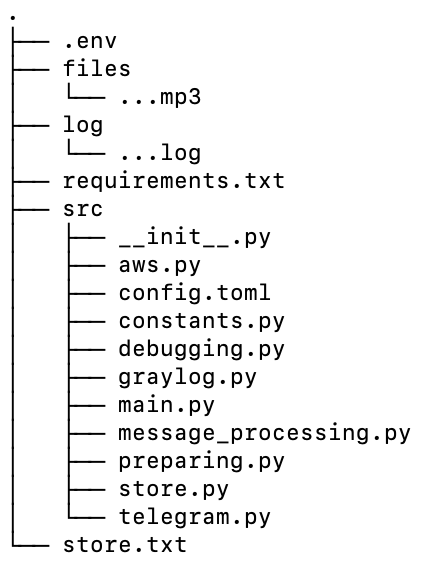
\includegraphics[scale=0.7]{dateisystem}
\caption{Gekürzte Ausgabe des Programms 'tree' im Basisverzeichnis.}
\label{fig:dateisystem}
\end{figure}

In absteigender Reihenfolge: die Datei '.env' beinhaltet sensible Zugangsdaten für die verschiedenen Dienste und wird nicht in das öffentliche GitHub-Repository hochgeladen. Das Verzeichnis 'files' dient als Zwischenspeicher für anfallende Audiodateien, welche aus den eingehenden Sprachnachrichten extrahiert wurden oder per Sprachsynthese erzeugt wurden. Im Verzeichnis 'log' werden die textbasierten Protokolle der Software gespeichert. Zu jedem Start der Software wird eine neue Datei mit dem aktuellen Datum erzeugt. Die Inhalte der Dateien entsprechen der Konsolenausgabe mit der Ausnahme, dass sensible Daten nur in der Konsolenausgabe ausgegeben werden. Die Datei requirements.txt dient als Informationsquelle für den Paketmanager pip, mit welchem die Abhängigkeiten aus dem Python Package Index installiert werden können. Sie beinhaltet Namen und Versionsnummern von externen Softwaremodulen. Der Ordner 'src' (Abkürzung für engl. 'source', zu deutsch 'Quelle') beinhaltet den Quellcode. Die Datei '\_\_init\_\_.py' ist notwendig für die Moduldefinitionen in Python und hat keinen Inhalt. Weitere Dateien im Quellcode-Verzeichnis entsprechen den Modulen und werden in \autoref{sec:module} detaillierter erläutert. Schließlich wird die Datei 'store.txt' für die Persistierung des Werts für den Parameter 'update\_id' der Telegram Bot API verwendet.

\subsection{Module}
\label{sec:module}

Der Quellcode wurde in mehrere Module aufgeteilt:

\begin{itemize}
\item \lstinline{main}: Dieses Modul enthält die Hauptfunktion des Programms und startet die Vorbereitung und den Übergang in den Regelbetrieb.
\item \lstinline{debugging}: Dieses Modul enthält die für die Fehlersuche notwendigen Funktionen. Siehe \autoref{sec:protokollierung}.
\item \lstinline{preparing}: Dieses Modul enthält die für den Startvorgang notwendigen Funktionen, welche nicht Teil eines anderen Moduls sind. Siehe \autoref{sec:startvorgang}
\item \lstinline{telegram}: Dieses Modul enthält Funktionen für den Zugriff auf die Telegram-API. Die HTTP-Abfragen werden mit dem Modul \lstinline{requests} \footnote{\url{https://pypi.org/project/requests/}} durchgeführt. Weiterhin sind Funktionen für die Bearbeitung der Antworten der API enthalten. Die Authentifizierung an der API erfolgt über nur dem Entwickler bekannte Zugriffssschlüssel, welche vom Telegram-Bot \lstinline{@BotFather} ausgestellt werden.
\item \lstinline{aws}: Dieses Modul enthält Funktionen für den Zugriff auf AWS. Für die Kommunikation mit der API wird das SDK für die Programmiersprache Python des AWS-Teams \lstinline{boto3} verwendet. Die Verwendung der Python SDK für AWS 'boto3' gegenüber einer 'low-level' Implementierung der HTTP-Abfragen mit dem Modul \lstinline{requests} bringt mehrere Vorteile, beispielsweise in der Sitzungsverwaltung. Weiterhin bietet die boto3-Bibliothek die Möglichkeit, für ausgesuchte Dienste einen mehr objektorientierten und von API-Funktionen abstrahierten Zugriff zu verwenden \footnote{\url{https://boto3.amazonaws.com/v1/documentation/api/latest/guide/resources.html}}.
\item \lstinline{constants}: Dieses Modul beinhaltet Variablen, mit welchen der Ablauf des Programms gesteuert werden kann (beispielsweise können detaillierte Meldungen zum Programmablauf aktiviert oder bestimmte Telegram-Benutzer für den Zugriff auf den Bot autorisiert werden). Des Weiteren sind Variablen als Platzhalter Teil des Moduls, welche zur Laufzeit mit Objektdefinitionen der boto3-Bibliothek überschrieben werden. Dies ermöglicht einen durchgehenden Zugriff auf die AWS-API ohne wiederkehrende Authentifizierungen.
\item \lstinline{graylog}: Dieses Modul beinhaltet Funktionen für den Zugriff auf die Graylog API. Der Zugriff erfolgt ähnlich wie beim Modul \lstinline{telegram} über das Paket \lstinline{requests}. Aus Sicherheitsgründen werden verschiedene Zugangsschlüssel für die Autorisierung und Authentifizierung verwendet \footnote{\url{https://docs.graylog.org/docs/rest-api}}. Der 'access token' (zu deutsch '(dauerhafter) Zugriffsschlüssel') entspricht den Anmeldedaten an der Graylog Webschnittstelle. Mit diesem können zeitlich befristete 'session token' (zu deutsch 'Sitzungsschlüssel') generiert werden. Die Software erkennt anhand der von der API zurückgegebenen Fehlermeldung automatisch, wenn ein nicht gültiger 'session token' verwendet wurde und beantragt in diesem Fall einen neuen.
\item \lstinline{message_processing}: Dieses Modul enthält interne Funktionen, welche für die Verarbeitung der erhaltenen Nachrichtentexte vorgesehen sind. 
\item \lstinline{store}: Dieses Modul enthält Funktionen, welche für die Persistierung von Informationen notwendig sind. Die Telegram-API verwendet einen Zähler, welcher für jede Aktualisierung um einen Schritt inkrementiert wird. Ruft der Client Aktualisierungen von der API ab, erhält er den derzeitigen Stand als Wert der Variable 'update\_id' (vgl. \autoref{lst:bsp-telegram-api}, Zeile 7). Bei weiteren Anfragen an die API gibt der Client die Variable 'update\_id' an, um nur Aktualisierungen zu erhalten, die seit der letzten Abfrage eingetroffen sind (und daher einen höheren Wert der Variable 'update\_id' haben). Die Variable 'update\_id' wird nach jeder Abfrage in die Textdatei store.txt auf das lokale Dateisystem geschrieben.
\end{itemize}

\section{Protokollierung}
\label{sec:protokollierung}

Für die Protokollierung wurde ein selbstentwickeltes Programmmodul erweitert. Als Grundlage diente das Modul 'debugging' des GitHub-Repositorys 'Jomibe/wireguard-config-generator' \footnote{\url{https://github.com/Jomibe/wireguard-config-generator/blob/main/src/debugging.py}}. Das Repository enthält den Quellcode sowie die Dokumentation eines Softwareprojekts, welches im Rahmen des Moduls "Projekt" im Sommersemester 2022 an der Fachhochschule Südwestfalen implementiert wurde. Es wurde eine Software entwickelt, mit welcher die Konfigurationsdateien eines WireGuard VPN-Servers verwaltet werden können. Das Programm ermöglicht es unter anderem, die existierenden Konfigurationsdateien auf Syntax- und semantische Fehler zu prüfen und Konfigurationen für weitere VPN-Clients inkl. der Bestimmung von geeigneten Netzwerkkonfigurationen hinzuzufügen. Das Modul 'debugging' enthält Funktionen, welche für die Fehlersuche während der Laufzeit verwendet werden. In dem Modul wird die Funktion \lstinline{console()} implementiert, um die Ausgabe von Statusmeldungen auf der Konsole zentral zu koordinieren. 

Alle Statusmeldungen werden in einer Textdatei hinterlegt, wessen Pfad in der Datei 'config.py' konfiguriert wird. Ist der \lstinline{DEBUG}-Modus aktiv, erscheinen alle Meldungen zusätzlich auf der Konsole. Ist die Fehlermeldung mit dem Parameter \lstinline{secret} gekennzeichnet, erfolgt keine Protokollierung in der Textdatei. Werden Meldungen auf der Konsole ausgegeben, werden diese gemäß dem Schweregrad farblich markiert. Dazu wird das Modul 'colorama' \footnote{\url{https://pypi.org/project/colorama/}} verwendet.

Im Anhang befinden sich zwei Listings mit den Konsolenausgaben des Programms beim Start (\autoref{log-start}) und beim Verarbeiten einer eingegangenen Nachricht (\autoref{log-msg}).

\section{Startvorgang}
\label{sec:startvorgang}

Das Modul \lstinline{main} enthält die Methode \lstinline{main()}, welche den Startpunkt des Programms darstellt. In der Vorbereitungsphase (vgl. \autoref{sec:grundsaetzlicher-aufbau}) wird zuerst die Programmbibliothek \lstinline{colorama} initialisiert. Dies ist notwendig, um die Steuerung der Farbausgabe auf der Konsole an das zur Laufzeit verwendete Betriebssystem anzupassen \footnote{\url{https://github.com/tartley/colorama\#initialisation}}. Nach der Initialisierung wird die Funktion \lstinline{prepare()} aus dem Modul \lstinline{preparing} aufgerufen. Diese Funktion stellt einen sogenannten 'hook' dar, welcher sämtliche Prüfungen vor Beginn des Regelbetriebs beinhaltet. Wird eine Prüfung nicht erfolgreich abgeschlossen, gibt \lstinline{prepare()} den Wert \lstinline{False} zurück und der Programmablauf wird nach Ausgabe einer detaillierten Fehlermeldung abgebrochen. Falls kein Fehlerstatus zurückgegeben wird, wird zum Regelbetrieb übergegangen. Dieser besteht aus einer Endlosschleife, in welcher die Funktion \lstinline{check_updates()} des Moduls \lstinline{telegram} aufgerufen wird.

\section{Regelbetrieb}

Im Regelbetrieb wird die Funktion \lstinline{getUpdates} der Telegram-API mittels 'long-polling' aufgerufen. Der Wert für den Ablauf der HTTP-Anfrage kann mittels des Parameters \lstinline{TELEGRAM_LONG_POLL_TIMEOUT} verändert werden, standardmäßig sind 30 Sekunden eingestellt.

Eingehende Nachrichten werden in Echtzeit erkannt und weiterverarbeitet. Falls mehrere Nachrichten vorliegen (dies kommt vor, wenn die Software für längere Zeit nicht mit der Telegram-API verbunden war und in der Zwischenzeit mehrere Nachrichten an den Bot gesendet wurden), wird jeweils nur eine Nachricht verarbeitet, da die Variable 'update\_id' nur um jeweils einen Schritt (statt um die Anzahl der neuen Nachrichten) inkrementiert wird. Zuerst wird anhand der Chat ID (vgl. \autoref{lst:bsp-telegram-api}, Zeile 18) ermittelt, ob der Benutzer durch den Administrator für die Verwendung des Bots freigegeben wurde. Hierzu wird der Wert mit der Liste \lstinline{constants.AUTHORIZED_CHAT_IDS} verglichen. Bei positivem Ergebnis erfolgt die Verarbeitung der Nachrichteninhalte: anhand des Aufbaus des JSON-Objekts wird ermittelt, ob es sich um eine Text- oder Sprachnachricht handelt. Der Text einer Nachricht wird direkt durch die Funktion \lstinline{message_processing.process_text_message} verarbeitet. Handelt es sich um eine Sprachnachricht, wird zuerst die Audiodatei von der Telegram Bot-API bezogen und auf dem lokalen Dateisystem abgelegt. Danach erfolgt der Transkriptionsprozess in einer weiteren Funktion, welche den ermittelten Text in einer Zeichenkette zurückgibt. Schließlich wird der Text ebenfalls durch die Funktion \lstinline{message_processing.process_text_message} verarbeitet.

\subsection{Optimierung der Antwortzeit}

Die Bedienung eines Systems mittels Sprache erfordert eine umfangreichere Benutzerführung als die Bedienung eines textbasierten Systems über einen Bildschirm und eine Tastatur. Beim Aufruf einer Webseite in langsamen Netzwerken bietet der Bildschirm durch die Anzeige des Webbrowsers mit diversen Statuselementen eine dauerhafte Möglichkeit für den Benutzer zu prüfen, ob die gewünschte Anfrage eingegangen ist und verarbeitet wird. Eine nur auf Sprache basierende Bedienung bietet keine äquivalente Möglichkeit, dem Benutzer eine Statusübersicht bis zum Abschluss der Anfrage zur Verfügung zu stellen. Um Missverständnisse vorzubeugen und die Bedienung komfortabel zu gestalten, muss das System eine Rückmeldung innerhalb eines durch den Menschen als nicht zu lang empfundenen Zeitraums zurückgeben \cite{response-time}. Bei der Entwicklung fiel auf, dass die Dauer zwischen Absenden der Sprachnachricht und Erhalt einer Antwort mit den Ergebnissen bis zu 30 Sekunden betrug. Diese Antwortzeit ist nicht akzeptabel. Eine Analyse des Programmablaufs ergab, dass die Transkription und die Sprachsynthese (der Text-To-Speech Prozess) einen Großteil der benötigten Antwortzeit verursachten. Beide Prozesse wurden optimiert, sodass die Verarbeitungszeit der Transkription von 15 Sekunden auf etwa zwei Sekunden und die der Sprachsynthese von 10 Sekunden auf weniger als eine Sekunde verkürzt werden konnte.

Die Zeit von der Erkennung neuer Nachrichten durch den Bot bis zum Abschluss des Versands der Sprachnachricht mit der Antwort beträgt nun etwa fünf Sekunden.

\subsubsection{Transkription}

Die Transkription durch Amazon Transcribe wurde optimiert, indem statt der boto3-Bibliothek das Amazon Transcribe Streaming SDK \footnote{\url{https://github.com/awslabs/amazon-transcribe-streaming-sdk}} verwendet wurde. Hierdurch ergaben sich neue Möglichkeiten für die Übermittlung der Audionachricht und des ermittelten Texts durch den Einsatz von HTTP-Streams und asynchronen Funktionen. Mit der boto3-Bibliothek war eine Verarbeitung in Echtzeit nicht möglich. Die Audiodatei musste zuerst in einen S3-Speicher hochgeladen werden. Eine Möglichkeit für die direkte Zuführung der Datei besteht nicht. Im Anschluss musste ein Auftrag in Amazon Transcribe über das \lstinline{client}-Objekt in \lstinline{constants.aws_transcribe_obj} erstellt und die Datei im S3-Speicher damit verknüpft werden. Danach wurde der Auftrag durch AWS verarbeitet. Die Möglichkeit eines 'callbacks' oder der Verwendung von 'long-polling' (vgl. \autoref{sec:telegram-getting-updates}) bestand nicht, daher musste die AWS-API mittels 'polling' durchgehend erneut kontaktiert werden, bis der Auftrag abgeschlossen war. Der transkribierte Text wurde nach der Bearbeitung des Auftrags durch AWS in einem S3-Speicher als JSON-Objekt in einer Textdatei hinterlegt. Nachdem die Datei von S3 bezogen wurde, konnte der Text durch die Software weiterverarbeitet werden.

Der Vorgang wurde durch die Verwendung des Transcribe SDK optimiert, indem die vom Hersteller bereitgestellte Vorlage für eine asynchrone Verarbeitung \footnote{\url{https://github.com/awslabs/amazon-transcribe-streaming-sdk/blob/v0.6.0/examples/simple\_file.py}} umgeschrieben wurde. Im Gegensatz zur oben beschriebenen Verwendung von boto3 werden die Audiodaten hierbei direkt Amazon Transcribe über einen HTTP-Stream zugeführt. Dazu wird die zu übertragende Datei, welche sich nach dem Bezug von der Telegram Bot-API auf dem lokalen Dateisystem befindet, mittels des Python Moduls 'aiofile' \footnote{https://pypi.org/project/aiofile/} in Blöcke mit einer Größe von 16 Kilobyte aufgeteilt und in mehreren Paketen an die AWS-API übertragen. Bereits während der Übertragung und dem Erhalt der ersten Blöcke durch AWS beginnt die Transkription. Die Software implementiert gleichzeitig einen 'event handler', welcher Daten von der AWS API in Echtzeit empfängt und nach Abschluss eines Satzes (dies ist an dem Parameter \lstinline{is_partial}, zu deutsch \lstinline{ist_unvollständig} erkennbar), den Text der Software zuführt und die weitere Verarbeitung durch Abschluss der Funktion auslöst.

Die Entwickler des Transcribe SDK weisen darauf hin, dass sich die Software bislang in einem sehr frühen Entwicklungsstadium befindet. Zum Zeitpunkt der Entwicklung wurde die Version 0.6.0 verwendet. Um die Funktionsweise des Bots nicht durch die Abhängigkeit zum Entwicklungsstand der Transcribe SDK zu gefährden, besteht die Möglichkeit, zwischen der klassischen Transkription mit boto3 und der Echtzeit-Transkription mit dem Konfigurationsparameter \lstinline{ENABLE_FAILSAFE_TRANSCRIPTION} zu wechseln.

\subsubsection{Sprachsynthese}

Die Dauer des Text-To-Speech Vorgangs wurde in ähnlicher Weise optimiert wie die der Transkription. Die dazu notwendigen Funktionen waren bereits in der boto3-Bibliothek enthalten. Statt der Funktion \lstinline{start_speech_synthesis_task} wird die Funktion \lstinline{synthesize_speech} verwendet. Dadurch entfällt die Notwendigkeit, die durch AWS erzeugte Audiodatei aus einem S3-Speicher herunterladen zu müssen. Nachdem der TTS-Auftrag zuvor gestartet wurde, musste dieser ebenfalls mittels 'polling' überwacht werden. Der umzuwandelnde Text wird der API weiterhin als Zeichenkette übergeben. Mit der Funktion \lstinline{synthesize_speech} ist es nun möglich, die Audiodatei aus einem Stream in eine Datei auf dem lokalen Dateisystem zu schreiben. 

\subsection{Verarbeitung des Nachrichtentexts}

Die weitere Verarbeitung des Nachrichtentexts erfolgt nach dem zuvor definierten Modell (vgl. \autoref{sec:syntax}) aus Produktkategorie, Eigenschaft und Zeitraum. Die Schlüsselwörter für die drei zu erkennenden Werte können über \lstinline{constants.KEYWORDS*} festgelegt werden. Voreingestellt für die Produktkategorie sind ‘Typ' und 'Kategorie', für die Eigenschaft die Schlüsselwörter 'bezüglich' und 'in Sachen' und für den Zeitraum 'Zeitraum' und 'seit'. Die Software ermittelt beim Startvorgang, wie viele Wörter die Bezeichnungen für Produktkategorie und Eigenschaft maximal umfassen (hat eine Produktkategorie die Eigenschaften 'Unerreichbarkeit und 'Interne Fehler', entspricht die maximale Länge der Bezeichnungen von Eigenschaften der Anzahl zwei). Die Texterkennung prüft nun im ersten Schritt, ob die eingegangene Nachricht jeweils ein Schlüsselwort für die Produktkategorie, Eigenschaft und den Zeitraum enthält. Im nächsten Schritt werden die auf die Schlüsselwörter folgenden Wörter für die Weiterverarbeitung erfasst. Dabei werden so viele Wörter gespeichert, wie beim Startvorgang ermittelt. Zur Erläuterung:

\begin{lstlisting}[caption={Auszug aus der Datei config.toml}, label=config-toml, xleftmargin=6mm]
[Webserver]
"Zugriffe" = "http_response_code: 200"
"Interne Fehler" = "http_response_code:[500 TO 599]"
\end{lstlisting}

Die maximale Länge von Bezeichnungen der Produktkategorie ist \textbf{1}. Die maximale Länge von Bezeichnungen der Eigenschaft ist \textbf{2}.

Nachricht: "Ich benötige Informationen zu Systemen vom \textit{Typ} \underline{Webserver} \textit{bezüglich} \underline{Zugriffe \textit{Zeitraum}} 24 Stunden"

\begin{itemize}
\item Produktkategorie: Schlüsselwort \textit{Typ}, folgende \textbf{1} Wörter: \underline{Webserver}
\item Eigenschaft: Schlüsselwort \textit{bezüglich}, folgende \textbf{2} Wörter: \underline{Zugriffe Zeitraum}
\end{itemize}

Nun prüft die Software, ob zu den erfassten Daten Einträge in der Datei 'config.toml' bestehen. Im obigen Fall führt \underline{Webserver} durch direkte Übereinstimmung mit der ersten TOML-Sektion zu einem Fund. Im Folgenden werden die Eigenschaften der ermittelten Produktkategorie auf Übereinstimmung mit \underline{Zugriffe Zeitraum} verglichen. Eine solche Eigenschaft existiert nicht. Besteht der erfasste Wert aus mehr als einem Wort, wird das letzte Wort entfernt. Aus \underline{Zugriffe Zeitraum} wird \underline{Zugriffe}. Damit gibt es eine direkte Übereinstimmung zu Zeile 2 des obigen Listings. Die Software entnimmt der Datenstruktur den Suchbegriff \lstinline{http_response_code: 200} und startet eine Abfrage an die Graylog-API.

Der Zeitraum wird in ähnlicher Form ermittelt. Hierbei wird die Anzahl der zu erfassenden Wörter auf die Anzahl zwei festgelegt. Das zweite Wort entspricht der Zeiteinheit, das erste Wort entspricht der Anzahl der Zeiteinheit. Die Texterkennung der Anzahl erkennt sowohl Zahlen als auch Zahlwörter ("ein", "eine", "letzte"). Wurde eine Übereinstimmung bei der Erkennung beider Werte erreicht, wird die Anzahl der Sekunden berechnet (zwei Tage entsprechen 60s*60*24*2 = 172800s) und der Anfrage an die Graylog-API angehängt.

\begin{lstlisting}[caption={Anfrage der Software an Graylog mit den ermittelten Daten}, label=config-toml, xleftmargin=6mm]
GET http://10.10.12.1:9000/api/views/search/messages

{
"streams": [
"000000000000000000000001"
],
"timerange": [
"relative",
{
"range": "172800"
}
],
"query_string": { "type":"elasticsearch", "query_string":"http_response_code: 200" }
}
\end{lstlisting}

Der Benutzer erhält eine spezifische Fehermeldung für den Fall, dass

\begin{itemize}
\item die Produktkategorie nicht ermittelt werden konnte
\item die Produktkategorie ermittelt werden konnte, aber die Eigenschaft nicht
\item der Zeitraum nicht ermittelt werden konnte
\end{itemize}

Die Antwort der Graylog-API erfolgt in einem JSON-Objekt, welches sämtliche auf den Suchbegriff und Zeitraum passende Ereignisse beinhaltet. Die Software bestimmt die Anzahl der Ereignisse und gibt diese an den Benutzer zurück. Im Anschluss wird die nächste Nachricht verarbeitet.

\subsubsection{Implementierung von Aliasdefinitionen}

Um die Erkennung von Begriffen und die Erweiterbarkeit des Zuordnungssystems in der Datei 'config.toml' zu verbessern, wurden Alias-Bezeichnungen für Produktkategorien und Eigenschaften implementiert. Ein Alias einer Produktkategorie übernimmt sämtliche Eigenschaften der Zieldefinition. Ein Alias einer Eigenschaft übernimmt den Suchbegriff der Zieldefinition. Im folgenden Listing führt die Eigenschaft Besucher der Produktkategorie eins zum Suchbegriff \lstinline{http_response_code: 200}

\begin{lstlisting}[caption={Aliasdefinitionen in der Datei config.toml}, label=alias-config-toml, xleftmargin=6mm]
[Webserver]
"Besucher Zugriffe" = "http_response_code: 200"
"Besucher" = "::ALIAS::Besucher Zugriffe"

[Eins]
"::ALIAS::" = "Webserver"
\end{lstlisting}
